\documentclass[12pt,a4paper]{article}
\usepackage[utf8]{vietnam}
\usepackage{amsmath,amssymb}
\usepackage{geometry}
\geometry{top=1.3cm,bottom=1.2cm,left=1.4cm,right=1.4cm,headheight=15pt,headsep=12pt,footskip=18pt}
\usepackage{tikz}
\usepackage{xcolor}
\usepackage{enumerate}
\usepackage{graphicx}
\usepackage[version=4]{mhchem}
\usepackage{fancyhdr}
\usepackage{ex_test}


\renewcommand{\baselinestretch}{0.95}
\setlength{\parskip}{0pt}

\definecolor{hfRed}{RGB}{211,47,47}
\definecolor{hfGreen}{RGB}{139,195,144}

\pagestyle{fancy}
\fancyhf{}
\fancyhead[L]{\small\itshape\color{hfRed} Tài liệu lưu hành nội bộ}
\fancyhead[R]{\small\itshape\color{hfRed} Thầy \textbf{TRẦN VĂN THẠNH} - 0777.470.803}
\renewcommand{\headrulewidth}{0.8pt}
\renewcommand{\headrule}{\hbox to\headwidth{\color{hfGreen}\leaders\hrule height \headrulewidth\hfill}}

\fancyfoot[L]{\small\itshape\color{hfRed} CS1: 6/15 Nguyễn Hoàng, P. Kim Long, TP Huế \quad|\quad CS2: 24 Đặng Thái Thân, TP Huế}
\fancyfoot[R]{\small\bfseries\color{hfRed} Trang \thepage}
\renewcommand{\footrulewidth}{0.8pt}
\renewcommand{\footrule}{\hbox to\headwidth{\color{hfGreen}\leaders\hrule height \footrulewidth\hfill}}

\fancypagestyle{firstpage}{
  \fancyhf{}
  \renewcommand{\headrulewidth}{0pt}
  \fancyfoot[L]{\small\itshape\color{hfRed} CS1: 6/15 Nguyễn Hoàng, P. Kim Long, TP Huế \quad|\quad CS2: 24 Đặng Thái Thân, TP Huế}
  \fancyfoot[R]{\small\bfseries\color{hfRed} Trang \thepage}
  \renewcommand{\footrulewidth}{0.8pt}
  \renewcommand{\footrule}{\hbox to\headwidth{\color{hfGreen}\leaders\hrule height \footrulewidth\hfill}}
}

\renewcommand{\loigiai}[1]{%
  \par\smallskip\noindent{\color{blue!80!black}\textbf{Lời giải:}}\ #1\par\smallskip
}
\renewcommand{\True}{\bfseries\color{red!80!black}}

\begin{document}
\thispagestyle{firstpage}

\noindent
\begin{minipage}[t]{0.40\textwidth}
	\centering\fontsize{9.5pt}{12pt}\selectfont
	\textbf{SỞ GD\&ĐT THỪA THIÊN HUẾ}\\
	\textbf{TRƯỜNG THPT CAO THẮNG}\\
	\textbf{Mã đề thi: 103}
\end{minipage}\hfill
\begin{minipage}[t]{0.58\textwidth}
	\centering\small
	\textbf{ĐỀ KIỂM TRA CUỐI KÌ II, NĂM HỌC 2023--2024}\\
	\textbf{MÔN: HÓA HỌC 10}\\
	\textbf{\color{red!80!black}(HƯỚNG DẪN CHẤM VÀ LỜI GIẢI CHI TIẾT)}
\end{minipage}

\smallskip
\noindent
\textit{Cho biết Nguyên tử khối của: $\ce{Na}=23$; $\ce{K}=39$; $\ce{Al}=27$; $\ce{Br}=80$; $\ce{Cl}=35{,}5$; $\ce{I}=127$; $\ce{O}=16$; $\ce{H}=1$.}

\smallskip
\noindent
\textbf{A. PHẦN TRẮC NGHIỆM (28 CÂU, 07 ĐIỂM).}

\Opensolutionfile{ans}[ans-gv]

\begin{ex}
Enthalpy tạo thành của một chất là
\choice
{nhiệt kèm theo phản ứng trong điều kiện chuẩn}
{\True nhiệt kèm theo phản ứng tạo thành 1 mol chất đó từ các đơn chất bền nhất}
{nhiệt kèm theo phản ứng tạo thành 1 mol chất đó từ các hợp chất bền nhất}
{nhiệt kèm theo phản ứng trong quá trình đẳng áp}
\loigiai{
Enthalpy tạo thành ($\Delta_f H$) của một chất là lượng nhiệt kèm theo của phản ứng tạo thành 1 mol chất đó từ các đơn chất ở dạng bền nhất trong điều kiện đã cho.\\
\textbf{Chọn B.}
}
\end{ex}

\begin{ex}
Tiến hành các thí nghiệm sau:
\begin{enumerate}[(a)]
	\item Cho một mẩu đá vôi ($\ce{CaCO3}$) vào dung dịch $\ce{HCl}$.
	\item Cho $\ce{KBr}$ tác dụng với dung dịch $\ce{H2SO4}$ đặc nóng.
	\item Cho dung dịch $\ce{AgNO3}$ vào dung dịch $\ce{HI}$.
	\item Cho dung dịch $\ce{AgNO3}$ vào dung dịch $\ce{HF}$.
\end{enumerate}
Sau khi kết thúc thí nghiệm, số phản ứng xảy ra thuộc loại phản ứng oxi hóa -- khử là
\choice
{2}
{4}
{3}
{\True 1}
\loigiai{
(a) $\ce{CaCO3 + 2HCl -> CaCl2 + CO2 ^ + H2O}$ (phản ứng trao đổi, không phải oxi hóa -- khử).\\
(b) $\ce{2KBr + 2H2SO4}\text{ (đặc, nóng)} \ce{-> K2SO4 + Br2 + SO2 ^ + 2H2O}$ ($\ce{Br^-}$ tăng lên $\ce{Br^0}$, $\ce{S^{+6}}$ giảm xuống $\ce{S^{+4}}$ $\rightarrow$ là phản ứng oxi hóa -- khử).\\
(c) $\ce{AgNO3 + HI -> AgI v + HNO3}$ (phản ứng trao đổi, không phải oxi hóa -- khử).\\
(d) $\ce{AgNO3 + HF}$ không xảy ra phản ứng vì $\ce{AgF}$ tan tốt trong nước.\\
Vậy chỉ có 1 phản ứng oxi hóa -- khử (thí nghiệm b).\\
\textbf{Chọn D.}
}
\end{ex}

\begin{ex}
Cho 6 gam $\ce{Zn}$ hạt vào một cốc đựng dung dịch $\ce{H2SO4}$ 4M (dư) ở nhiệt độ thường. Nếu giữ nguyên các điều kiện khác, chỉ biến đổi một trong các điều kiện sau đây:
\begin{enumerate}[(1)]
	\item Thay 6 gam $\ce{Zn}$ hạt bằng 6 gam $\ce{Zn}$ bột.
	\item Thay dung dịch $\ce{H2SO4}$ 4 M bằng dung dịch $\ce{H2SO4}$ 2 M.
	\item Thực hiện phản ứng ở nhiệt độ cao hơn (khoảng $50^\circ\text{C}$).
	\item Dùng thể tích dung dịch $\ce{H2SO4}$ 4 M gấp đôi ban đầu.
\end{enumerate}
Những biến đổi nào làm tăng tốc độ phản ứng?
\choice
{\True (1), (3)}
{(1), (3), (4)}
{(2), (3), (4)}
{(1), (2), (3), (4)}
\loigiai{
(1) Dùng $\ce{Zn}$ bột làm tăng diện tích tiếp xúc $\rightarrow$ tăng tốc độ phản ứng.\\
(2) Giảm nồng độ dung dịch $\ce{H2SO4}$ từ 4M xuống 2M $\rightarrow$ giảm tốc độ phản ứng.\\
(3) Tăng nhiệt độ lên $50^\circ\text{C}$ $\rightarrow$ tăng tốc độ phản ứng.\\
(4) Thể tích tăng gấp đôi nhưng nồng độ không đổi và axit đã dư sẵn $\rightarrow$ tốc độ phản ứng không đổi.\\
Do đó các biến đổi làm tăng tốc độ là (1) và (3).\\
\textbf{Chọn A.}
}
\end{ex}

\begin{ex}
Dẫn 2,479 lít (đkc) khí chlorine vào 200 ml dung dịch sodium hydroxide 1,5M ở nhiệt độ thường. Biết phản ứng xảy ra hoàn toàn, khối lượng chất tan có trong dung dịch sau phản ứng là
\choice
{7,45 gam}
{13,30 gam}
{\True 17,30 gam}
{5,85 gam}
\loigiai{
$n_{\ce{Cl2}} = \dfrac{2{,}479}{24{,}79} = 0{,}1\text{ mol}$; $n_{\ce{NaOH}} = 0{,}2 \times 1{,}5 = 0{,}3\text{ mol}$.\\
Phương trình: $\ce{Cl2 + 2NaOH -> NaCl + NaClO + H2O}$.\\
So sánh tỉ lệ: $\dfrac{n_{\ce{Cl2}}}{1} = 0{,}1 < \dfrac{n_{\ce{NaOH}}}{2} = 0{,}15 \rightarrow \ce{NaOH}$ dư ($0{,}3 - 0{,}2 = 0{,}1\text{ mol}$).\\
Khối lượng các chất tan sau phản ứng:
\begin{itemize}
	\item $m_{\ce{NaCl}} = 0{,}1 \times 58{,}5 = 5{,}85\text{ gam}$.
	\item $m_{\ce{NaClO}} = 0{,}1 \times 74{,}5 = 7{,}45\text{ gam}$.
	\item $m_{\ce{NaOH}\text{ dư}} = 0{,}1 \times 40 = 4{,}00\text{ gam}$.
\end{itemize}
Tổng khối lượng chất tan $= 5{,}85 + 7{,}45 + 4{,}00 = 17{,}30\text{ gam}$.\\
\textbf{Chọn C.}
}
\end{ex}

\begin{ex}
Có phản ứng: $\ce{CH4(g) + 2O2(g) ->[t^\circ] CO2(g) + 2H2O(g)}$\\
Cho biết giá trị năng lượng liên kết của một số liên kết:
\begin{center}
\begin{tabular}{|l|c|c|c|c|}
\hline
Liên kết & C--H & O--H & C=O & O=O \\ \hline
$E_b$ (kJ/mol) & 413 & 467 & 745 & 498 \\ \hline
\end{tabular}
\end{center}
Biến thiên enthalpy chuẩn của phản ứng trên là
\choice
{\True $-710\text{ kJ}$}
{$+668\text{ kJ}$}
{$-978\text{ kJ}$}
{$-434\text{ kJ}$}
\loigiai{
$\Delta_r H^\circ_{298} = \sum E_b(\text{chất đầu}) - \sum E_b(\text{sản phẩm})$\\
$\sum E_b(\text{đầu}) = 4 \cdot E_b(\text{C-H}) + 2 \cdot E_b(\text{O=O}) = 4 \times 413 + 2 \times 498 = 2648\text{ kJ}$.\\
$\sum E_b(\text{sp}) = 2 \cdot E_b(\text{C=O}) + 4 \cdot E_b(\text{O-H}) = 2 \times 745 + 4 \times 467 = 3358\text{ kJ}$.\\
$\Delta_r H^\circ_{298} = 2648 - 3358 = -710\text{ kJ}$.\\
\textbf{Chọn A.}
}
\end{ex}

\begin{ex}
Phản ứng nào dưới đây chứng minh tính khử của các ion halide?
\choice
{$\ce{2HCl + CuO -> CuCl2 + H2O}$}
{$\ce{BaCl2 + H2SO4 -> BaSO4 + 2HCl}$}
{\True $\ce{2HBr + H2SO4 -> Br2 + SO2 + 2H2O}$}
{$\ce{HI + NaOH -> NaI + H2O}$}
\loigiai{
Trong phản ứng $\ce{2HBr + H2SO4 -> Br2 + SO2 + 2H2O}$, số oxi hóa của $\ce{Br}$ tăng từ $-1$ lên $0$ trong $\ce{Br2}$, thể hiện tính khử của ion $\ce{Br-}$.\\
\textbf{Chọn C.}
}
\end{ex}

\begin{ex}
Hydrogen halide có nhiệt độ sôi cao nhất là
\choice
{$\ce{HCl}$}
{$\ce{HI}$}
{$\ce{HBr}$}
{\True $\ce{HF}$}
\loigiai{
$\ce{HF}$ có nhiệt độ sôi cao bất thường trong dãy hydrogen halide do giữa các phân tử $\ce{HF}$ hình thành liên kết hydrogen liên phân tử bền.\\
\textbf{Chọn D.}
}
\end{ex}

\begin{ex}
Nhận định nào sau đây đúng?
\choice
{Bất cứ phản ứng nào cũng cần tăng áp suất để tăng tốc độ phản ứng}
{Chất xúc tác là chất làm tăng tốc độ phản ứng và biến mất sau khi phản ứng kết thúc}
{\True Chất xúc tác làm tăng tốc độ phản ứng nhưng vẫn được bảo toàn về chất và lượng khi kết thúc phản ứng}
{Bất cứ phản ứng nào cũng cần chất xúc tác để tăng tốc độ phản ứng}
\loigiai{
Chất xúc tác làm tăng tốc độ phản ứng nhưng không bị tiêu hao (vẫn được bảo toàn về lượng và chất) sau khi phản ứng kết thúc.\\
\textbf{Chọn C.}
}
\end{ex}

\begin{ex}
Dựa vào phương trình nhiệt hóa học của phản ứng:
\[\ce{CO2(g) -> CO(g) + 1/2 O2(g)} \quad \Delta_r H^\circ_{298} = +280\text{ kJ}\]
Giá trị $\Delta_r H^\circ_{298}$ của phản ứng: $\ce{2CO2(g) -> 2CO(g) + O2(g)}$ là
\choice
{\True $+560\text{ kJ}$}
{$-420\text{ kJ}$}
{$+140\text{ kJ}$}
{$-1120\text{ kJ}$}
\loigiai{
Hệ số tỉ lượng của phản ứng thứ hai gấp 2 lần phản ứng thứ nhất $\rightarrow \Delta_r H^\circ_{298} = 2 \times (+280\text{ kJ}) = +560\text{ kJ}$.\\
\textbf{Chọn A.}
}
\end{ex}

\begin{ex}
Trong tự nhiên, các halogen
\choice
{tồn tại ở cả dạng đơn chất và hợp chất}
{chỉ tồn tại ở dạng muối halide}
{chỉ tồn tại ở dạng đơn chất}
{\True chỉ tồn tại ở dạng hợp chất}
\loigiai{
Do có hoạt tính hóa học mạnh (tính oxi hóa mạnh) nên các halogen trong tự nhiên không tồn tại ở dạng đơn chất mà chỉ tồn tại ở dạng hợp chất.\\
\textbf{Chọn D.}
}
\end{ex}

\begin{ex}
Phát biểu \textbf{không} chính xác là
\choice
{Trong tất cả các hợp chất, fluorine chỉ có số oxi hóa -1}
{\True Trong tất cả các hợp chất, các halogen chỉ có số oxi hóa là -1}
{Trong hợp chất với hydrogen và kim loại, các halogen luôn thể hiện số oxi hóa là -1}
{Tính oxi hóa của halogen giảm dần từ fluorine đến iodine}
\loigiai{
Ngoài fluorine chỉ có số oxi hóa $-1$, các halogen khác ($\ce{Cl, Br, I}$) trong hợp chất với các nguyên tố có độ âm điện lớn hơn còn có các số oxi hóa dương $+1, +3, +5, +7$. Do đó phát biểu B là không chính xác.\\
\textbf{Chọn B.}
}
\end{ex}

\begin{ex}
Ý nghĩa của hệ số nhiệt độ Van't Hoff ($\gamma$) là
\choice
{\True giá trị của $\gamma$ càng lớn thì ảnh hưởng của nhiệt độ đến tốc độ phản ứng càng mạnh}
{giá trị của $\gamma$ càng lớn thì tốc độ phản ứng càng giảm}
{giá trị của $\gamma$ càng lớn thì ảnh hưởng của nhiệt độ đến tốc độ phản ứng càng yếu}
{giá trị của $\gamma$ càng lớn thì tốc độ phản ứng càng tăng}
\loigiai{
Hệ số $\gamma$ cho biết tốc độ phản ứng tăng lên bao nhiêu lần khi nhiệt độ tăng thêm $10^\circ\text{C}$. Do đó, $\gamma$ càng lớn thì ảnh hưởng của nhiệt độ đến tốc độ phản ứng càng mạnh.\\
\textbf{Chọn A.}
}
\end{ex}

\begin{ex}
Dung dịch dùng để nhận biết các ion halide là
\choice
{$\ce{NaOH}$}
{quỳ tím}
{$\ce{HCl}$}
{\True $\ce{AgNO3}$}
\loigiai{
Dung dịch $\ce{AgNO3}$ tạo kết tủa đặc trưng với các ion halide: $\ce{AgCl}$ trắng, $\ce{AgBr}$ vàng nhạt, $\ce{AgI}$ vàng đậm.\\
\textbf{Chọn D.}
}
\end{ex}

\begin{ex}
Trong các phản ứng hoá học, để chuyển thành anion, nguyên tử của các nguyên tố halogen đã nhận hay nhường bao nhiêu electron?
\choice
{Nhường đi 1 electron}
{\True Nhận thêm 1 electron}
{Nhận thêm 2 electron}
{Nhường đi 7 electron}
\loigiai{
Cấu hình electron lớp ngoài cùng của halogen là $ns^2np^5$, có 7 electron nên dễ nhận thêm 1 electron để đạt cấu hình bát cú bền vững: $\ce{X + 1e -> X-}$.\\
\textbf{Chọn B.}
}
\end{ex}

\begin{ex}
Chuẩn bị 3 ống nghiệm, các dung dịch có cùng nồng độ 0,1M. Tiến hành thí nghiệm theo các bước:
\begin{itemize}
	\item Bước 1: Cho vào mỗi ống nghiệm khoảng 2 mL dung dịch các chất như hình vẽ:
\end{itemize}
\begin{center}
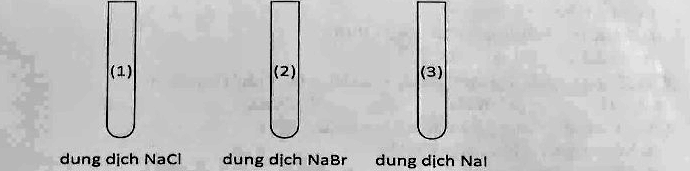
\includegraphics[width=6.5cm]{images_crop/fig_cau15_ongnghiem.png}
\end{center}
\begin{itemize}
	\item Bước 2: Cho vào mỗi ống nghiệm khoảng 1 mL nước chlorine.
	\item Bước 3: Thêm tiếp vào mỗi ống nghiệm vài giọt dung dịch $\ce{AgNO3}$.
\end{itemize}
Cho các phát biểu sau:
\begin{enumerate}[(1)]
	\item Cả ba ống nghiệm đều xuất hiện kết tủa trắng ở bước 2.
	\item Sau bước 3, chỉ có ống nghiệm (1) thu được kết tủa trắng.
	\item Từ hiện tượng quan sát được có thể kết luận tính oxi hoá của chlorine mạnh hơn của bromine và iodine.
	\item Dung dịch ở ống (1) không thể phản ứng với nước bromine.
\end{enumerate}
Số phát biểu đúng là
\choice
{\True 2}
{3}
{1}
{4}
\loigiai{
(1) Sai, ở bước 2 không có kết tủa nào xuất hiện.\\
(2) Sai, ở bước 3 sau khi $\ce{Cl2}$ phản ứng tạo $\ce{NaCl}$ thì các ống nghiệm đều có ion $\ce{Cl-}$ tạo kết tủa trắng $\ce{AgCl}$.\\
(3) Đúng, vì $\ce{Cl2}$ oxi hóa được $\ce{Br-}$ thành $\ce{Br2}$ và $\ce{I-}$ thành $\ce{I2}$.\\
(4) Đúng, vì bromine có tính oxi hoá yếu hơn chlorine nên không phản ứng với muối $\ce{NaCl}$.\\
Vậy có 2 phát biểu đúng là (3) và (4).\\
\textbf{Chọn A.}
}
\end{ex}

\begin{ex}
Cho các biến đổi sau:
\begin{enumerate}[(1)]
	\item Đun nóng chất tham gia.
	\item Thêm chất xúc tác phù hợp.
	\item Pha loãng dung dịch.
	\item Giảm nhiệt độ.
	\item Tăng nhiệt độ.
	\item Giảm diện tích bề mặt tiếp xúc.
	\item Tăng nồng độ chất phản ứng.
	\item Chia nhỏ chất phản ứng thành nhiều mảnh nhỏ.
\end{enumerate}
Có bao nhiêu biến đổi làm tăng tốc độ phản ứng?
\choice
{\True 5}
{7}
{6}
{4}
\loigiai{
Các biến đổi làm tăng tốc độ phản ứng là: (1) Đun nóng; (2) Thêm xúc tác; (5) Tăng nhiệt độ; (7) Tăng nồng độ; (8) Chia nhỏ chất phản ứng (tăng diện tích tiếp xúc). Tổng cộng có 5 biến đổi.\\
\textbf{Chọn A.}
}
\end{ex}

\begin{ex}
Cấu hình electron lớp ngoài cùng của nguyên tử các nguyên tố halogen là
\choice
{$ns^2np^6$}
{$ns^2np^4$}
{\True $ns^2np^5$}
{$ns^2np^3$}
\loigiai{
Nguyên tố halogen thuộc nhóm VIIA có 7 electron lớp ngoài cùng dạng $ns^2np^5$.\\
\textbf{Chọn C.}
}
\end{ex}

\begin{ex}
Trong phản ứng: $\ce{3Cu + 8HNO3 -> 3Cu(NO3)2 + 2NO + 4H2O}$. Số phân tử nitric acid ($\ce{HNO3}$) đóng vai trò chất oxi hóa là
\choice
{4}
{\True 2}
{8}
{6}
\loigiai{
Trong 8 phân tử $\ce{HNO3}$ tham gia: có 2 phân tử bị khử thành $\ce{NO}$ (đóng vai trò chất oxi hóa) và 6 phân tử tạo muối $\ce{Cu(NO3)2}$ (đóng vai trò môi trường).\\
\textbf{Chọn B.}
}
\end{ex}

\begin{ex}
Loại liên kết yếu được hình thành giữa nguyên tử H (đã liên kết với một nguyên tử có độ âm điện lớn, thường là F, O, N) với một nguyên tử khác (có độ âm điện lớn, thường là F, O, N) còn cặp electron hóa trị chưa tham gia liên kết là
\choice
{liên kết cộng hóa trị có cực}
{\True liên kết hydrogen}
{liên kết ion}
{liên kết cộng hóa trị không cực}
\loigiai{
Định nghĩa liên kết hydrogen.\\
\textbf{Chọn B.}
}
\end{ex}

\begin{ex}
Tốc độ của một phản ứng có dạng: $v = k \cdot C_A^x \cdot C_B^y$ (A, B là 2 chất khác nhau). Nếu tăng nồng độ chất A lên 2 lần, nồng độ chất B không đổi thì tốc độ phản ứng tăng 8 lần. Giá trị của x là
\choice
{6}
{\True 3}
{8}
{4}
\loigiai{
$\dfrac{v'}{v} = 2^x = 8 = 2^3 \Rightarrow x = 3$.\\
\textbf{Chọn B.}
}
\end{ex}

\begin{ex}
Yếu tố áp suất ảnh hưởng đến tốc độ phản ứng nào dưới đây?
\choice
{\True $\ce{2CO(g) + O2(g) -> 2CO2(g)}$}
{$\ce{Fe(s) + S(s) -> FeS(s)}$}
{$\ce{NaOH(aq) + HCl(aq) -> NaCl(aq) + H2O(l)}$}
{$\ce{NH4Cl(s) -> NH3(g) + HCl(g)}$}
\loigiai{
Áp suất chỉ ảnh hưởng đến tốc độ của phản ứng khi có chất tham gia phản ứng ở thể khí. Phản ứng A có $\ce{CO(g)}$ và $\ce{O2(g)}$ là chất phản ứng ở thể khí.\\
\textbf{Chọn A.}
}
\end{ex}

\begin{ex}
Trong phản ứng $\ce{Zn + CuSO4 -> ZnSO4 + Cu}$. Chất bị oxi hóa là
\choice
{$\ce{CuSO4}$}
{\True $\ce{Zn}$}
{$\ce{ZnSO4}$}
{$\ce{Cu}$}
\loigiai{
$\ce{Zn}$ có số oxi hóa tăng từ $0$ lên $+2$ $\rightarrow \ce{Zn}$ là chất khử $\rightarrow \ce{Zn}$ bị oxi hóa.\\
\textbf{Chọn B.}
}
\end{ex}

\begin{ex}
Đặc điểm chung của đơn chất halogen là
\choice
{Vừa có tính oxi hóa vừa có tính khử}
{\True Có tính oxi hóa mạnh}
{Tác dụng mạnh với nước}
{Ở điều kiện thường là chất khí}
\loigiai{
Các halogen đều có tính oxi hóa mạnh do có độ âm điện lớn, dễ nhận thêm 1 electron để đạt cấu hình electron bền vững.\\
\textbf{Chọn B.}
}
\end{ex}

\begin{ex}
Cho phương trình hóa học của phản ứng: $\ce{2A + B -> C}$. Biểu thức tính tốc độ tức thời của phản ứng là
\choice
{$v = k \cdot C_A \cdot C_B$}
{\True $v = k \cdot C_A^2 \cdot C_B$}
{$v = 2k \cdot C_A^2 \cdot C_B$}
{$v = k \cdot C_A \cdot C_B^2$}
\loigiai{
Theo định luật tác dụng khối lượng, biểu thức tốc độ phản ứng là $v = k \cdot C_A^2 \cdot C_B$.\\
\textbf{Chọn B.}
}
\end{ex}

\begin{ex}
Cho các phát biểu sau:
\begin{enumerate}[(1)]
	\item Nước Javel có khả năng tẩy màu và sát khuẩn.
	\item Cho $\ce{Cl2}$ vào dung dịch $\ce{NaOH}$ đun nóng ta thu được nước Javel.
	\item Hydrofluoric acid là acid yếu.
	\item Tính khử của các ion halide tăng dần theo thứ tự: $\ce{F-}$, $\ce{Cl-}$, $\ce{Br-}$, $\ce{I-}$.
	\item Khí chlorine ẩm và nước chlorine đều có tính tẩy màu.
\end{enumerate}
Trong các phát biểu trên, số phát biểu đúng là
\choice
{1}
{3}
{\True 4}
{2}
\loigiai{
(1) Đúng, $\ce{NaClO}$ có tính oxi hóa mạnh.\\
(2) Sai, ở nhiệt độ đun nóng thu được muối chlorate $\ce{NaClO3}$, không thu được nước Javel.\\
(3) Đúng, $\ce{HF}$ là acid yếu.\\
(4) Đúng, tính khử tăng dần từ $\ce{F-}$ đến $\ce{I-}$.\\
(5) Đúng, $\ce{HClO}$ sinh ra có tính tẩy màu.\\
Số phát biểu đúng là 4 gồm (1), (3), (4), (5).\\
\textbf{Chọn C.}
}
\end{ex}

\begin{ex}
Cho phương trình nhiệt hoá học:
\[\ce{2Al_{(s)} + Fe2O3_{(s)} -> Al2O3_{(s)} + 2Fe_{(s)}} \quad \Delta_r H^\circ_{298} = -851{,}5\text{ kJ}\]
Phản ứng này là phản ứng
\choice
{\True tỏa nhiệt}
{trao đổi}
{trung hòa}
{thu nhiệt}
\loigiai{
Do $\Delta_r H^\circ_{298} = -851{,}5\text{ kJ} < 0$ nên phản ứng tỏa nhiệt.\\
\textbf{Chọn A.}
}
\end{ex}

\begin{ex}
Trong phản ứng hoá học, tốc độ phản ứng
\choice
{tỉ lệ nghịch với nhiệt độ của phản ứng}
{\True tăng khi nhiệt độ của phản ứng tăng}
{giảm khi nhiệt độ của phản ứng tăng}
{không đổi khi nhiệt độ của phản ứng tăng}
\loigiai{
Khi tăng nhiệt độ, tốc độ chuyển động nhiệt của các hạt tăng lên làm tăng số va chạm hiệu quả $\rightarrow$ tốc độ phản ứng tăng.\\
\textbf{Chọn B.}
}
\end{ex}

\begin{ex}
“Bảo quản thức ăn trong tủ lạnh để thức ăn lâu bị ôi thiu”. Yếu tố nào đã ảnh hưởng đến tốc độ phản ứng trong tình huống thực tiễn trên?
\choice
{Diện tích bề mặt}
{\True Nhiệt độ}
{Chất xúc tác}
{Nồng độ}
\loigiai{
Nhiệt độ thấp trong tủ lạnh làm chậm tốc độ phản ứng ôi thiu thức ăn.\\
\textbf{Chọn B.}
}
\end{ex}

\Closesolutionfile{ans}

\vspace{0.3cm}
\noindent
\textbf{B. PHẦN TỰ LUẬN (03 CÂU, 03 ĐIỂM).}

\begin{ex}
Hoàn thành phương trình hóa học của các phản ứng sau:
\begin{enumerate}[a.]
	\item $\ce{Br2} + \dots \rightarrow \ce{KBr} + \ce{I2}$
	\item $\ce{KMnO4} + \dots \rightarrow \dots + \dots + \ce{Cl2} + \ce{H2O}$
	\item $\ce{Fe + Cl2 ->[t^\circ]} \dots$
	\item $\ce{Cl2 + NaOH ->[t^\circ] NaCl} + \dots + \ce{H2O}$
\end{enumerate}
\loigiai{
a. $\ce{Br2 + 2KI -> 2KBr + I2}$\\
b. $\ce{2KMnO4 + 16HCl -> 2KCl + 2MnCl2 + 5Cl2 ^ + 8H2O}$\\
c. $\ce{2Fe + 3Cl2 ->[t^\circ] 2FeCl3}$\\
d. $\ce{3Cl2 + 6NaOH ->[t^\circ] 5NaCl + NaClO3 + 3H2O}$
}
\end{ex}

\begin{ex}
Để hoà tan hết một mẫu $\ce{Al}$ trong dung dịch $\ce{HCl}$ ở $25^\circ\text{C}$ cần 36 phút. Cũng mẫu $\ce{Al}$ đó tan hết trong dung dịch acid nói trên ở $45^\circ\text{C}$ trong 4 phút. Hỏi để hoà tan hết mẫu $\ce{Al}$ đó trong dung dịch acid nói trên ở $60^\circ\text{C}$ thì cần thời gian bao nhiêu giây?
\loigiai{
Thời gian phản ứng tỉ lệ nghịch với tốc độ phản ứng:
\[\dfrac{v_{45}}{v_{25}} = \dfrac{t_{25}}{t_{45}} = \dfrac{36}{4} = 9\]
Theo quy tắc Van't Hoff:
\[\dfrac{v_{45}}{v_{25}} = \gamma^{\frac{45 - 25}{10}} = \gamma^2 = 9 \Rightarrow \gamma = 3\]
Tốc độ phản ứng ở $60^\circ\text{C}$ so với ở $45^\circ\text{C}$:
\[\dfrac{v_{60}}{v_{45}} = \gamma^{\frac{60 - 45}{10}} = 3^{1{,}5} = 3\sqrt{3} \approx 5{,}196\]
Thời gian hòa tan hết mẫu $\ce{Al}$ ở $60^\circ\text{C}$:
\[t_{60} = \dfrac{t_{45}}{3\sqrt{3}} = \dfrac{4\text{ phút}}{3\sqrt{3}} = \dfrac{240\text{ giây}}{3\sqrt{3}} = \dfrac{80}{\sqrt{3}} \approx 46{,}19\text{ giây}\]
\textbf{Đáp số:} Khoảng $46{,}2\text{ giây}$ (hoặc $46{,}19\text{ giây}$).
}
\end{ex}

\begin{ex}
Theo tính toán của các nhà khoa học, để phòng bệnh bướu cổ và một số bệnh khác, mỗi người cần bổ sung $1{,}5 \cdot 10^{-4}\text{ g}$ nguyên tố iodine mỗi ngày. Nếu lượng iodine đó chỉ được bổ sung từ muối iodised (còn gọi là muối iot, chứa 25g $\ce{KI}$ trong một tấn muối) thì mỗi người cần bao nhiêu gam muối mỗi ngày?
\loigiai{
Khối lượng mol của $\ce{KI}$: $M_{\ce{KI}} = 39 + 127 = 166\text{ g/mol}$.\\
Khối lượng nguyên tố iodine trong 25 gam $\ce{KI}$:
\[m_{\ce{I}} = 25 \times \dfrac{127}{166} \approx 19{,}1265\text{ gam}\]
Hàm lượng của iodine trong 1 tấn ($10^6\text{ gam}$) muối iodised:
\[\%m_{\ce{I}} = \dfrac{19{,}1265}{10^6} = 1{,}91265 \cdot 10^{-5}\text{ (g I / g muối)}\]
Khối lượng muối iodised cần dùng mỗi ngày để bổ sung $1{,}5 \cdot 10^{-4}\text{ gam}$ iodine là:
\[m_{\text{muối}} = \dfrac{1{,}5 \cdot 10^{-4}}{\%m_{\ce{I}}} = \dfrac{1{,}5 \cdot 10^{-4} \times 166 \times 10^6}{25 \times 127} = \dfrac{24900}{3175} \approx 7{,}84\text{ gam}\]
\textbf{Đáp số:} Khoảng $7{,}84\text{ gam}$ muối mỗi ngày.
}
\end{ex}

\begin{center}
\textbf{---------HẾT---------}
\end{center}

\end{document}
